% !TeX spellcheck = en_US
% !TeX encoding = UTF-8
% !TeX root = ../document.tex

\newcommand{\TSprime}{\ensuremath{\TS'}\xspace}
\newcommand{\ntrue}{\ensuremath{n_\text{true}}\xspace}
\newcommand{\nexp}{\ensuremath{n_\text{exp}}\xspace}
\newcommand{\nobs}{\ensuremath{n_\text{obs}}\xspace}
\newcommand{\sigmatrue}{\ensuremath{\sigma_\text{true}}\xspace}
\newcommand{\sigmaexp}{\ensuremath{\sigma_\text{exp}}\xspace}

\chapter{Additional Studies}
\section{Coverage Analysis}
In this chapter, we will show that the test statistic \TS introduced in \fref{sec:test_statistic} can be directly interpreted as $p$-value: $p = \TS$. We will refer to the definition and requirements of a $p$-value and show that \TS sufficiently fulfills those requirements.
Additionally, we will repeat the analysis with \TSprime, using a normal prior (as used in previous \acs{MUSiC} theses) instead of the log-normal term in \TS and compare the results.

A $p$-value is an indicator for the significance of a deviation, where a smaller $p$-value corresponds to a higher significance. The $p$-value of a result is compared to a significance threshold $\alpha$, which is fixed before the statistical analysis. If the observed $p$-value is smaller than $\alpha$, the null hypothesis is rejected. In our case, rejection of the null hypothesis corresponds to falsification of the \acl{SM} and thus the discovery of new physics. 

Both values are constructed in way that the null hypothesis is (incorrectly) rejected by chance with a probability of $\alpha$:
\begin{align}
	\Pr( H_0\:\text{rejected} | H_0 ) &= \alpha \\
    \label{eq:coverage_inequality}
    \Rightarrow \Pr( p < \alpha | H_0 ) &= \alpha
\end{align}
This equation is tested during the \emph{coverage analysis}.

\subsubsection{Procedure}
To test \fref{eq:coverage_inequality}, we construct pseudo experiments based on the null hypothesis $H_0$ and calculate the corresponding $p$-value, in this case \TS or \TSprime. After generating and examining sufficiently many pseudo experiments, we can determine the rate of significant findings and compare them to the claimed significance threshold:
\begin{equation}
	p_\text{true} = \frac{\text{number of pseudo-experiments where $p < \alpha$}}{n_\text{toys}} = \Pr(p < \alpha | H_0)
    \label{eq:coverage}
\end{equation}

The pseudo experiments are based on \acs{MUSiC}'s null hypothesis: 
We assume that there is a constant probability that events end up in a particular region, and thus a constant true mean value \ntrue. 
We also assume that this true mean value is only known up to an expected event yield, \nexp.
The way that \nexp is derived from \ntrue differs between \TS and \TSprime: For \TS, \nexp is drawn from a log-normal probability density, \TSprime  will use a normal distribution instead.

Additionally, the physics process of performing a counting experiment has to be simulated: Here it is assumed that the event yield is caused by independent statistical processes with a fixed probability, thus the observed event yield follows a Poisson distribution around \ntrue.

The way that the assumed uncertainty enters the pseudo experiment also differs between \TS and \TSprime: For \TS, we recalculate the uncertainty after drawing \nexp in order to keep the relative uncertainty constant: $\sigmaexp = \frac{\nexp}{\ntrue} \sigmatrue$. For \TSprime, the absolute uncertainty is kept constant: $\sigmaexp = \sigmatrue$.
This has been argued by \cite[p. 78]{Schmitz:ModelUnspecificSearch}, a more rigorous discussion can be found in \fref{app:coverage_uncertainty}.

In the implementation, each pseudo-experiments begins with drawing \nexp from the probability density around \ntrue. At the same time, \nobs is drawn from a (discrete) Poisson distribution with a mean of \ntrue. From these two values, as well as the uncertainty \sigmaexp, \TS (or \TSprime) is calculated.

This process is repeated for $n_\text{toys}$ pseudo-experiments. An estimation for the true $p$ value is afterwards calculated using \fref{eq:coverage}, which yields the left hand side of \fref{eq:coverage_inequality}.

In order to state the so called "coverage value" for the tuple (\ntrue, \sigmatrue), both sides of  \fref{eq:coverage_inequality} are translated to $Z$-scores (see \fref{app:z_score}), resulting in $Z_\text{true} = Z(p_\text{true})$ representing the observed and $Z_\text{claim} = Z(\alpha)$ representing the claimed rate ob significant results.
The coverage is finally reported as
\begin{equation}
    \label{eq:coverage_value}
	\text{coverage} = Z_\text{true} - Z_\text{claim}.
\end{equation}
%or alternatively as 
%\begin{equation}
%    \text{coverage}' = \log_{10} %\left(\frac{p_\text{true}}{p_\text{claim}}\right)
%\end{equation}

\subsubsection{Interpretation of Results}
Three different result cases can arise, depending on the coverage value in \fref{eq:coverage_value}:
\begin{enumerate}
	\item $\text{coverage} = 0 \Leftrightarrow \Pr( H_0 \text{ rejected} | H_0 ) = \alpha$: This is the ideal case. It indicates the $p$-value performs according to its definition.
	\item $\text{coverage} < 0 \Leftrightarrow \Pr( H_0 \text{ rejected} | H_0 ) > \alpha$: The background hypothesis is rejected more often than with a probability of $\alpha$. This case is called "undercoverage" and corresponds to "liberal" behavior. The $p$-value overestimates the significance of deviations.
	\item $\text{coverage} > 0 \Leftrightarrow \Pr( H_0 \text{ rejected} | H_0 ) < \alpha$: The background hypothesis is not rejected in some cases where it should have been rejected. This effect is called "overcoverage" and corresponds to "conservative" behavior where the $p$-value underestimates the significance of deviations.
\end{enumerate}	

\subsubsection{Our Results}
Since the MUSiC $p$-value is required to cover a large range of possible \ntrue and relative uncertainty $\sigmatrue / \ntrue$ values, the coverage is evaluated on a two dimensional grid in this parameter space.
The computed results can be found in \fref{fig:coverage}.

\begin{figure}
    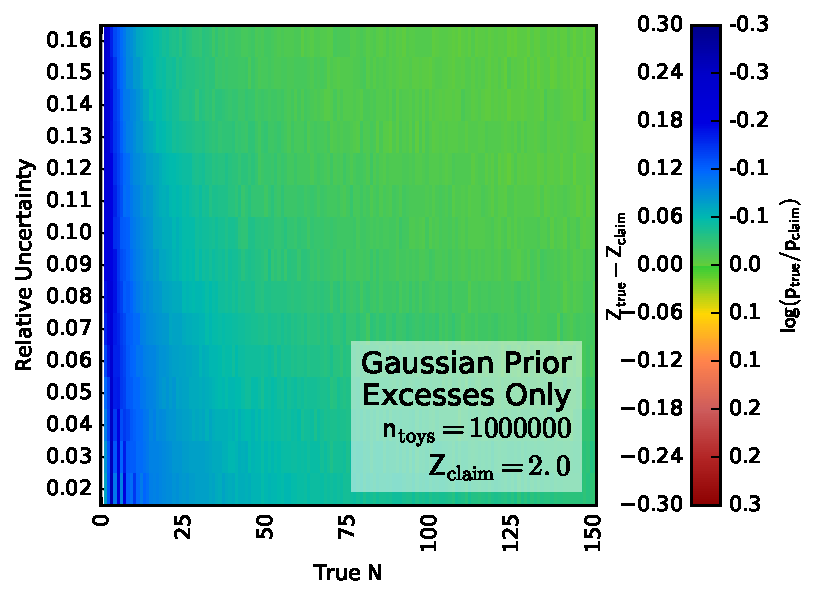
\includegraphics[width=\textwidth]{coverage/coverage_excess_normal_schmitz}
    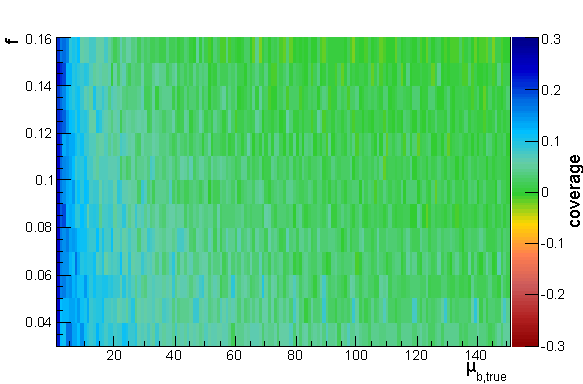
\includegraphics[width=\textwidth]{schmitz_coverage}
    \caption{Comparison of our results (top) with \cite{Schmitz:ModelUnspecificSearch} (bottom). The test settings as well as plotting options have been chosen to match. From visual inspection one can deduce that the results are very similar, which allows us to directly compare results from our implementation with the earlier thesis.}
    \label{fig:coverage_schmitz}
\end{figure}

\begin{figure}
    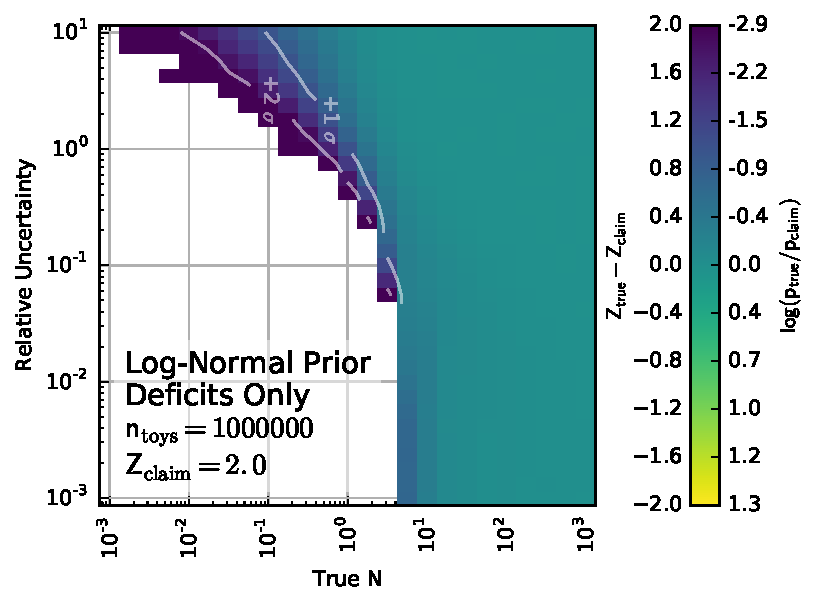
\includegraphics[width=\textwidth]{coverage/coverage_deficit_lognormal_log}
    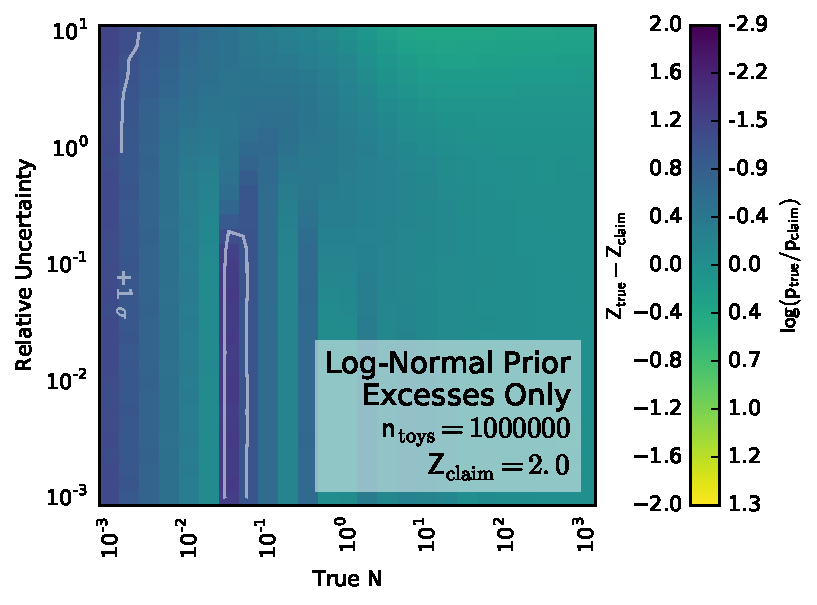
\includegraphics[width=\textwidth]{coverage/coverage_excess_lognormal_log}
    \caption{Results of the coverage analysis.}
    \label{fig:coverage}
\end{figure}

\begin{figure}
    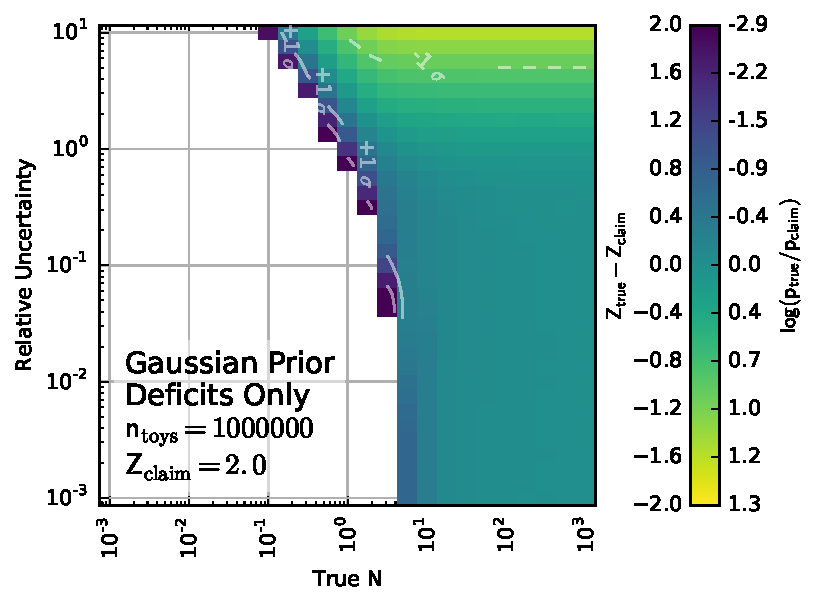
\includegraphics[width=\textwidth]{coverage/coverage_deficit_normal_log}
    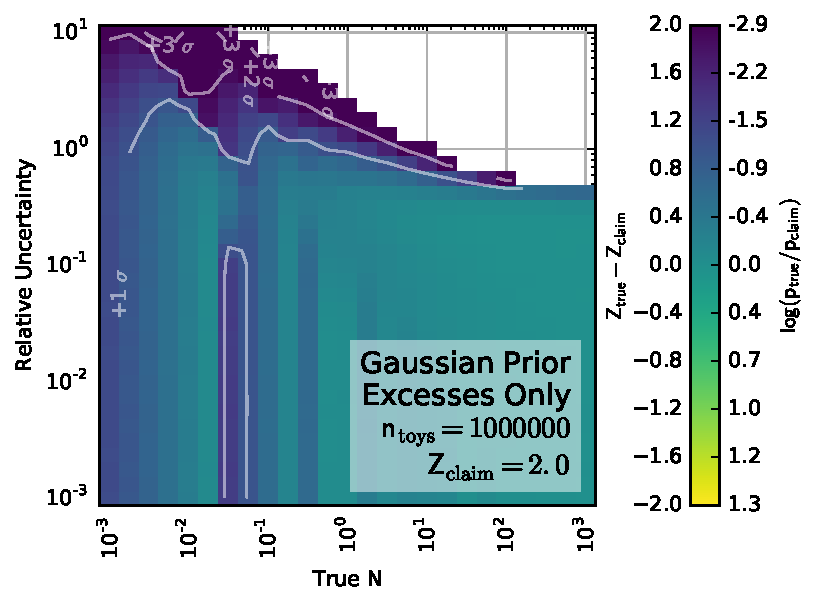
\includegraphics[width=\textwidth]{coverage/coverage_excess_normal_log}
    \caption{Results of the coverage analysis.}
    \label{fig:coverage2}
\end{figure}
\section{Log-Normal $p$-Value}

\section{A Global $p$-Value}
